\documentclass{beamer}

\usepackage[slovene]{babel} 
\usepackage[utf8]{inputenc}
\usepackage{graphicx}
\usepackage{subcaption}
\usepackage{geometry}
\usepackage{amssymb}
\usepackage{caption}
\usepackage{float}
\usepackage{wrapfig}
\usepackage{romannum}
\usepackage{physics}
\usepackage{amsmath,amsfonts,amsthm,bm} % Math packages
\usepackage[export]{adjustbox}

%\usetheme{CambridgeUS}

\title[Discretisation of 2D domains, bounded by NURBS]{Discretisation of 2D domains, bounded by NURBS curves}
\author[Andrej Kolar - Po{\v z}un]{Author: Andrej Kolar-Po{\v z}un \linebreak Mentor: Marjetka Knez}

\begin{document}
\begin{frame}
\titlepage
\end{frame}
\begin{frame}
\frametitle{NURBS}
\begin{itemize}
\item<1-> NURBS - Non Uniform Rational B-Splines.
\item<2-> B-Splines $N_{k,p}(\xi)$ basis for polynomial splines with prescribed smoothness.
\item<3-> B-Splines + Control points $\to$ B-Spline Curve (special case - Bézier curve).
\item<4-> $C(\xi) = \frac{\sum_{k=1}^n \textbf{P}_k w_k N_{k,p} (\xi)}{\sum_{k=1}^n w_k N_{k,p}(\xi)}$. 
\item<5-> Multipatch NURBS are also common.
\end{itemize}

\end{frame}
\begin{frame}
\frametitle{Problem description}
\begin{itemize}
\item<1-> $\partial \Omega = C(I)$ - simple and closed curve.
\item<2-> Goal - discretise $\Omega$. Obtain $X \subset \Omega$.
\item<3-> Motivation - Meshless methods and Monte Carlo.
\item<4-> Requirement 1: Algorithm takes $N$ or $h$ as input. 
\item<5-> Requirement 2: Quasiuniformness, quasirandomness.
\end{itemize}
\end{frame}
\begin{frame}
\frametitle{inRS}
\begin{itemize}
\item<1-> inRS\footnote{Sommariva, Vianello inRS: Implementing the indicator function of NURBS-shaped planar domains.} algorithm for calculating indicator function of $\Omega$.
\item<2-> $C(\xi) = \frac{\sum_{k=1}^n \textbf{P}_k w_k N_{k,p} (\xi)}{\sum_{k=1}^n w_k N_{k,p}(\xi)}$. 
\item<3-> Main idea - try reduce to the polygon case.
\item<4-> Divide $I$ into $I_k$ such that $C$ restricted to it is a pair of rational functions.
\item<5-> For each $I_k$, calculate the roots of the derivatives of the appropriate rational function.
\item<6-> For each $I_{k,j}$ find $a_{k,j} = \mathrm{min}_{I_{k,j}} \alpha_k(\xi)$
\item<7-> Cover $\partial \Omega$ by monotone boxes $\mathcal{B}_{k,j} = [a_{k,j},b_{k,j}] \times [c_{k,j} , d_{k,j}]$.
\end{itemize}
\end{frame}
\begin{frame}

\begin{itemize}
\item<2-> If $(x_0,y_0)$ outside global bounding box $\to$ also outside $\Omega$.
\item<3-> If $(x_0,y_0)$ outside monotone boxes - polygon case.
\item<4-> If inside one of the monotone boxes - polynomial solve.
\end{itemize}
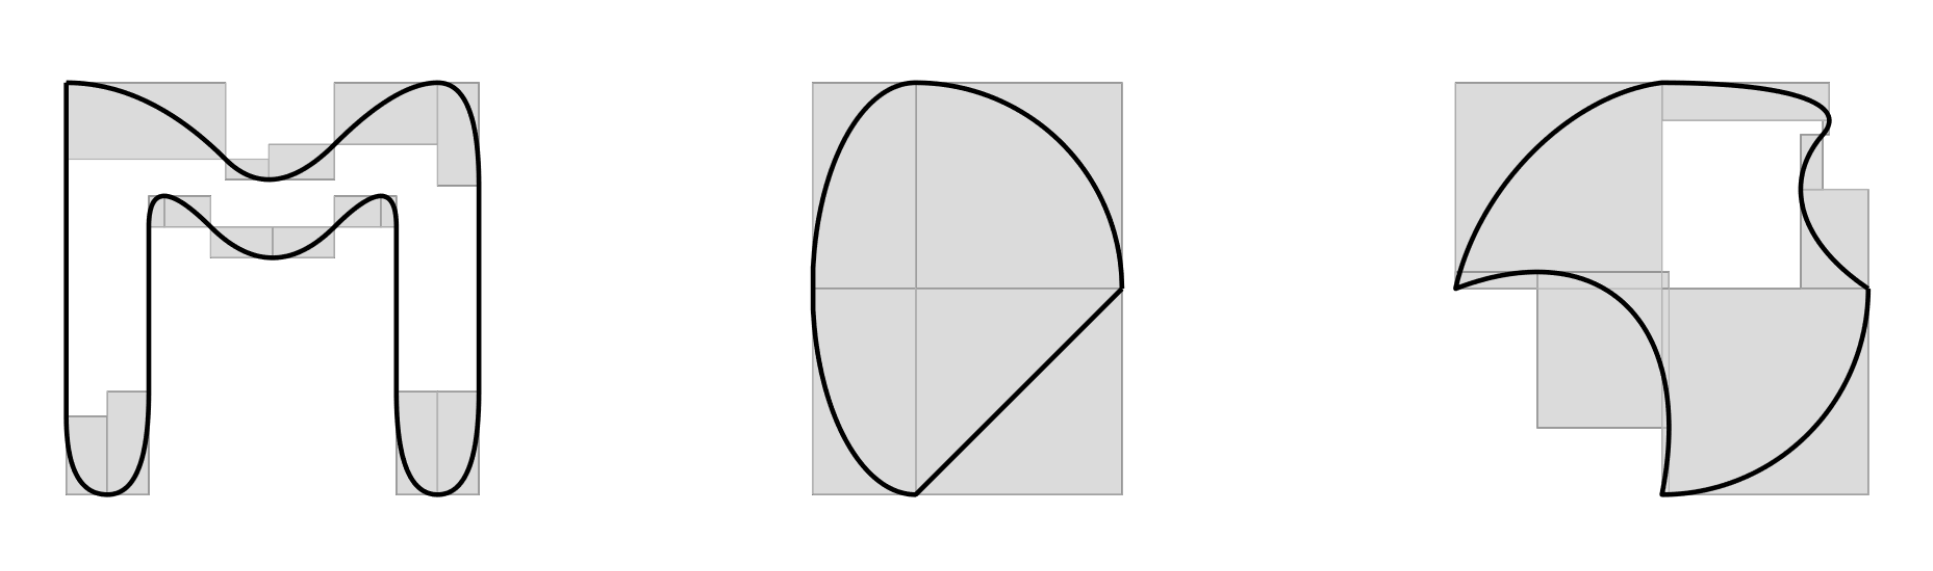
\includegraphics[width=\linewidth]{Slike/inRS_pokritje.png}
\end{frame}
\begin{frame}

\begin{itemize}
\item<1-> degenerate cases and multipatch.
\end{itemize}
\visible<2->{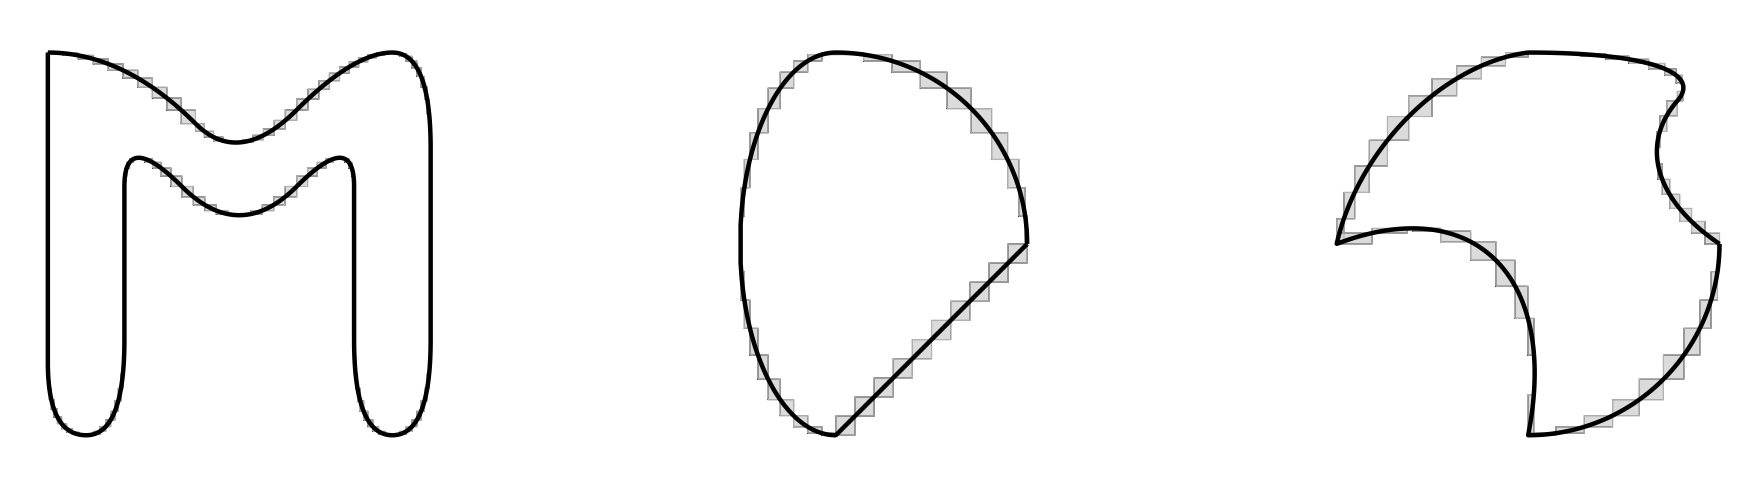
\includegraphics[width=\linewidth]{Slike/inRS_pokritje_fino.png}}
\end{frame}
\begin{frame}

\begin{itemize}
\item<1-> Halton nodes + rejection sampling
\end{itemize}
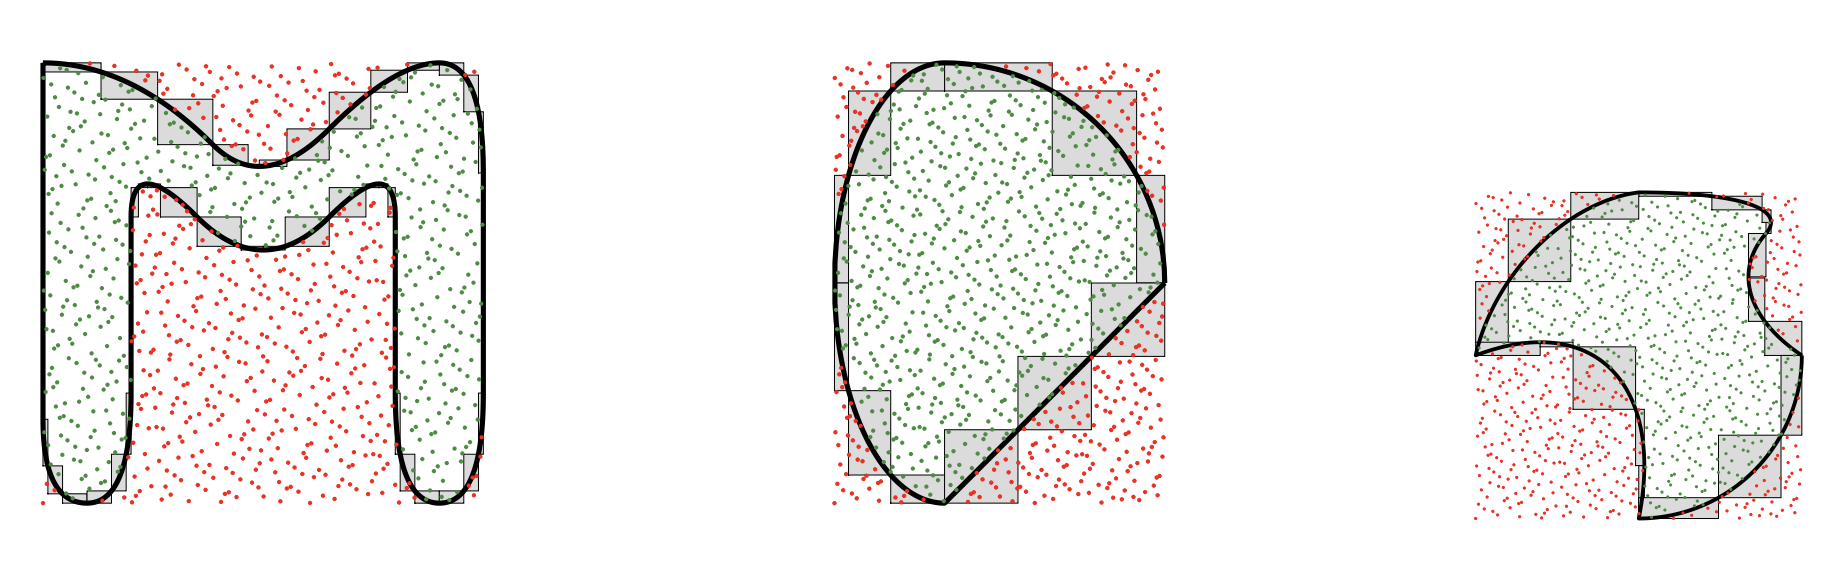
\includegraphics[width=\linewidth]{Slike/inRS_rezultat.png}
\end{frame}
\begin{frame}

\includegraphics[width=.3\linewidth]{Slike/inRS_example6.png}
\includegraphics[width=.3\linewidth]{Slike/inRS_example21.png}
\includegraphics[width=.3\linewidth]{Slike/inRS_example16.png}
\includegraphics[width=.3\linewidth]{Slike/inRS_example23.png}
\includegraphics[width=.3\linewidth]{Slike/inRS_example12.png}
\includegraphics[width=.3\linewidth]{Slike/inRS_example7.png}
\end{frame}
\begin{frame}
\frametitle{DIVG}
\begin{itemize}
\item<1-> DIVG\footnote{Slak, Kosec: On generation of node distributions for meshless PDE discretizations} - Dimension Independent Variable Density node Generation.
\item<3-> q - queue of active points, initially filled with seed points. Algorithm runs as long as it's non-empty.
\item<4-> At each step, pop q to get a point $x_0$, use it to generate new candidates.
\item<5-> Candidate is accepted if it's inside the domain and if it is far enough from already accepted points.
\item<6-> Algorithm is efficient with the help of a kd-tree.
\end{itemize}
\visible<2->{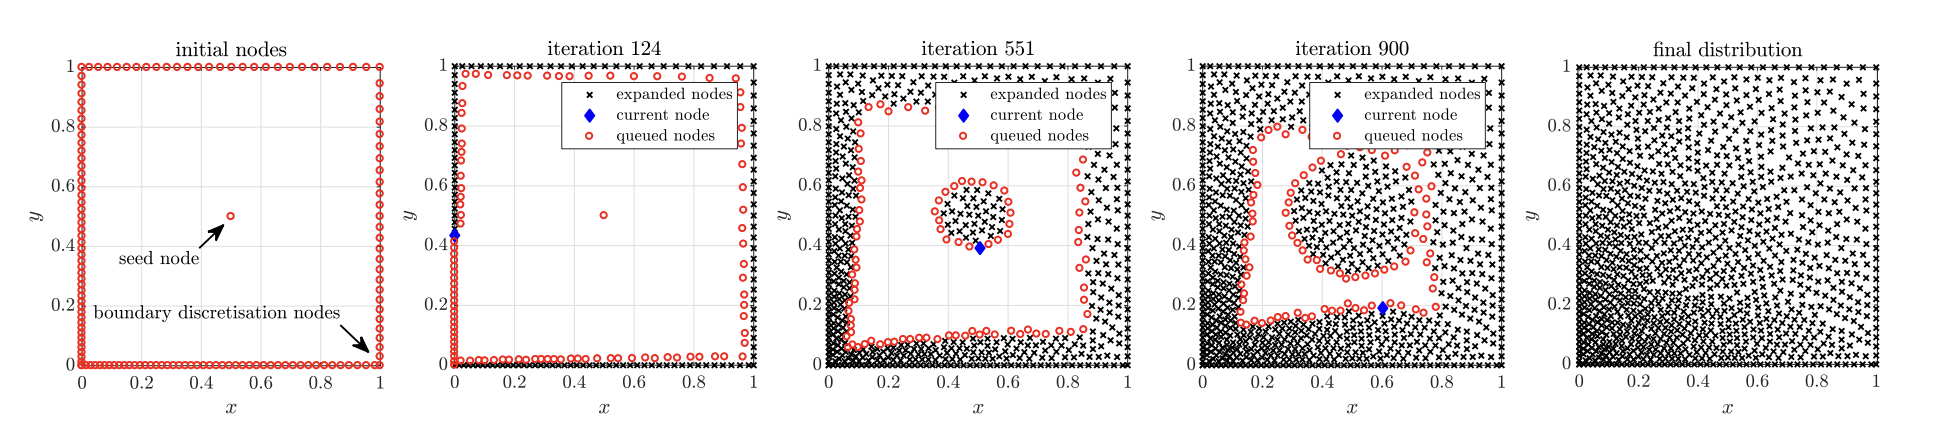
\includegraphics[width=\linewidth]{Slike/divg.png}}
\end{frame}
\begin{frame}
\includegraphics[width=\linewidth]{Slike/divgexplain.png}
\end{frame}
\begin{frame}
\begin{itemize}
\item<1-> sDIVG\footnote{Duh, Kosec, Slak: Fast variable density node generation on parametric surfaces with application to mesh-free methods} idea - use DIVG in the parameter space.
\end{itemize}
\visible<2->{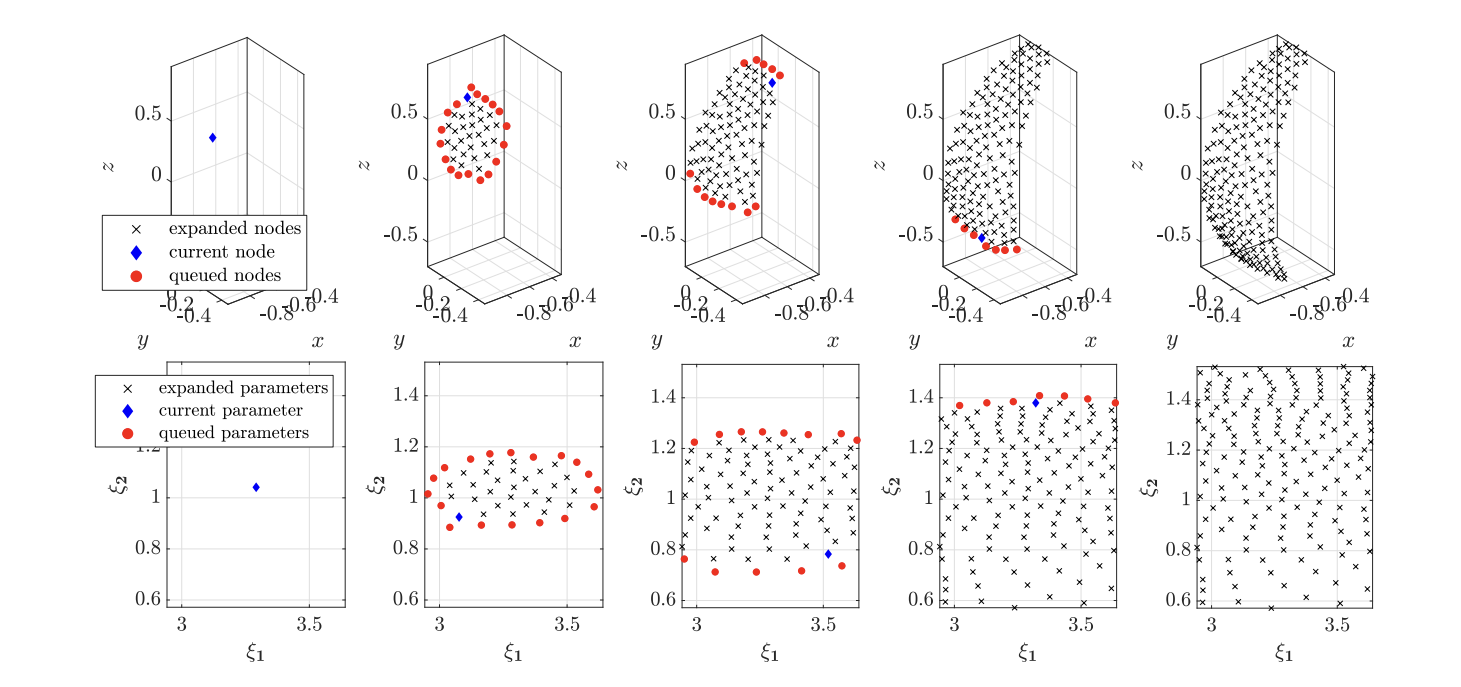
\includegraphics[width=\linewidth]{Slike/sdivg.png}}
\end{frame}
\begin{frame}
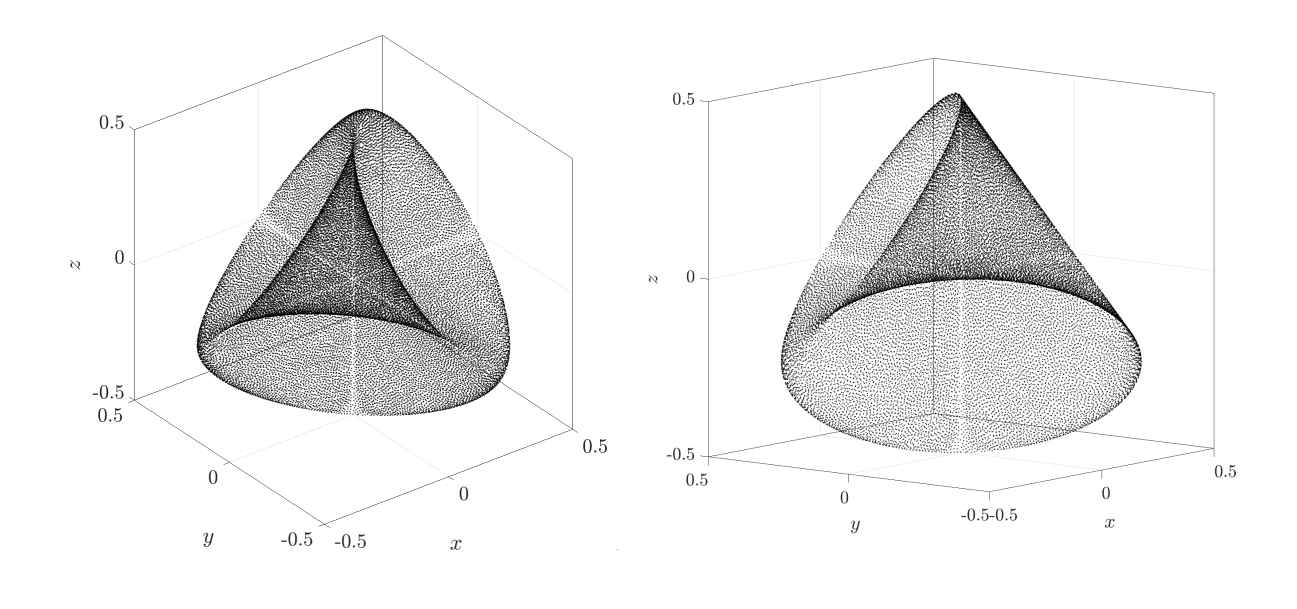
\includegraphics[width=\linewidth]{Slike/sdivgRoman.png}
\end{frame}
\begin{frame}
\begin{itemize}
\item<1-> NURBS-DIVG\footnote{Duh, Shankar, Kosec: Discretization of non-uniform rational B-spline (NURBS) models for meshless isogeometric analysis}
\item<2-> Multipatch - Discretise each patch seperately with sDIVG.
\end{itemize}
\visible<2->{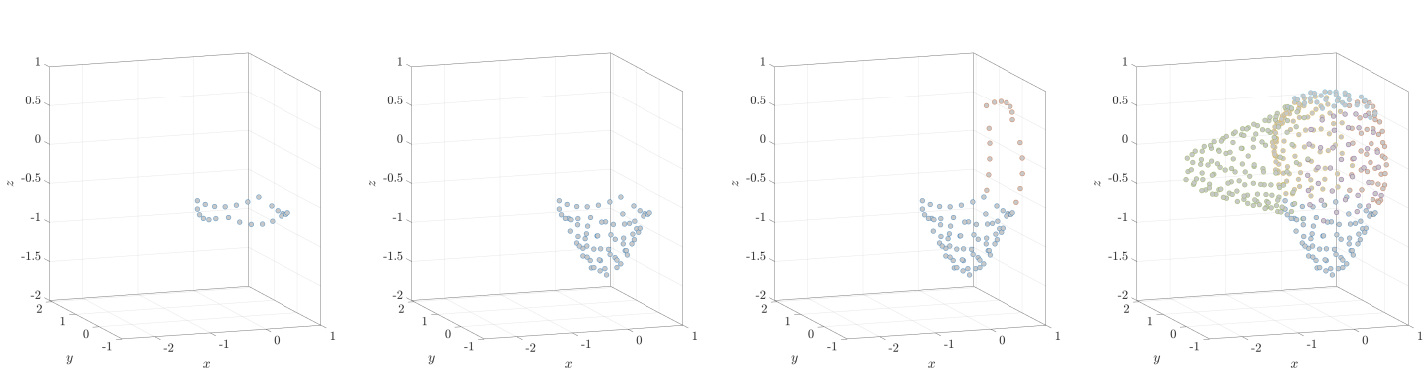
\includegraphics[width=\linewidth]{Slike/nurbsmultipatch.png}}
\end{frame}
\begin{frame}
\begin{itemize}
\item<1-> Interior check - $(\textbf{p}-\textbf{x})\cdot \textbf{n} > 0$
\item<3-> Improve accuracy with supersampling.
\end{itemize}
\visible<2->{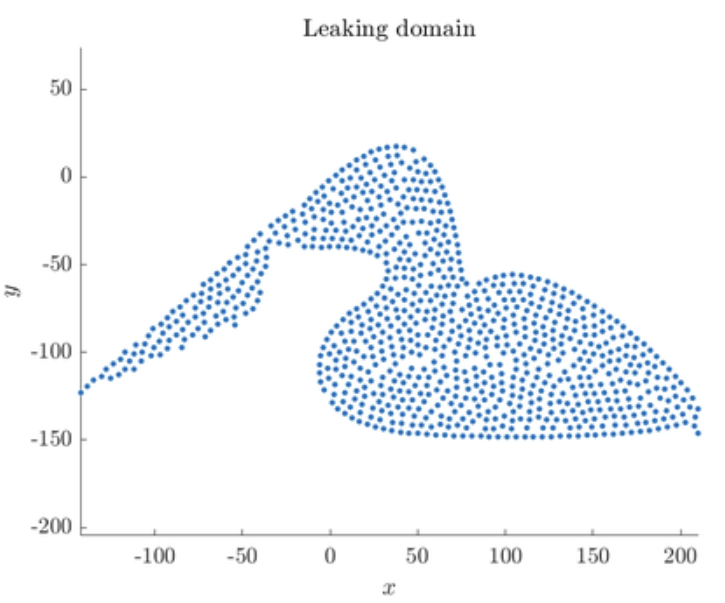
\includegraphics[width=.4\linewidth]{Slike/supersampling1.png}}
\visible<3->{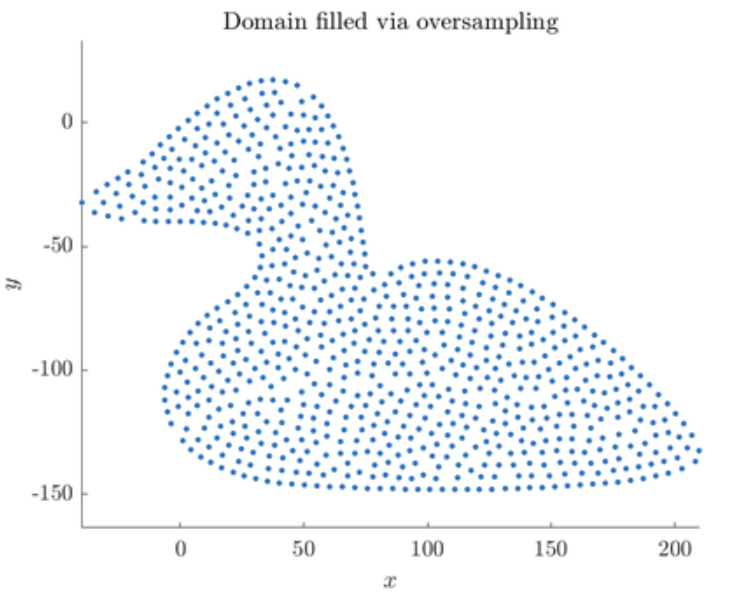
\includegraphics[width=.4\linewidth]{Slike/supersampling2.png}}
\end{frame}
\begin{frame}
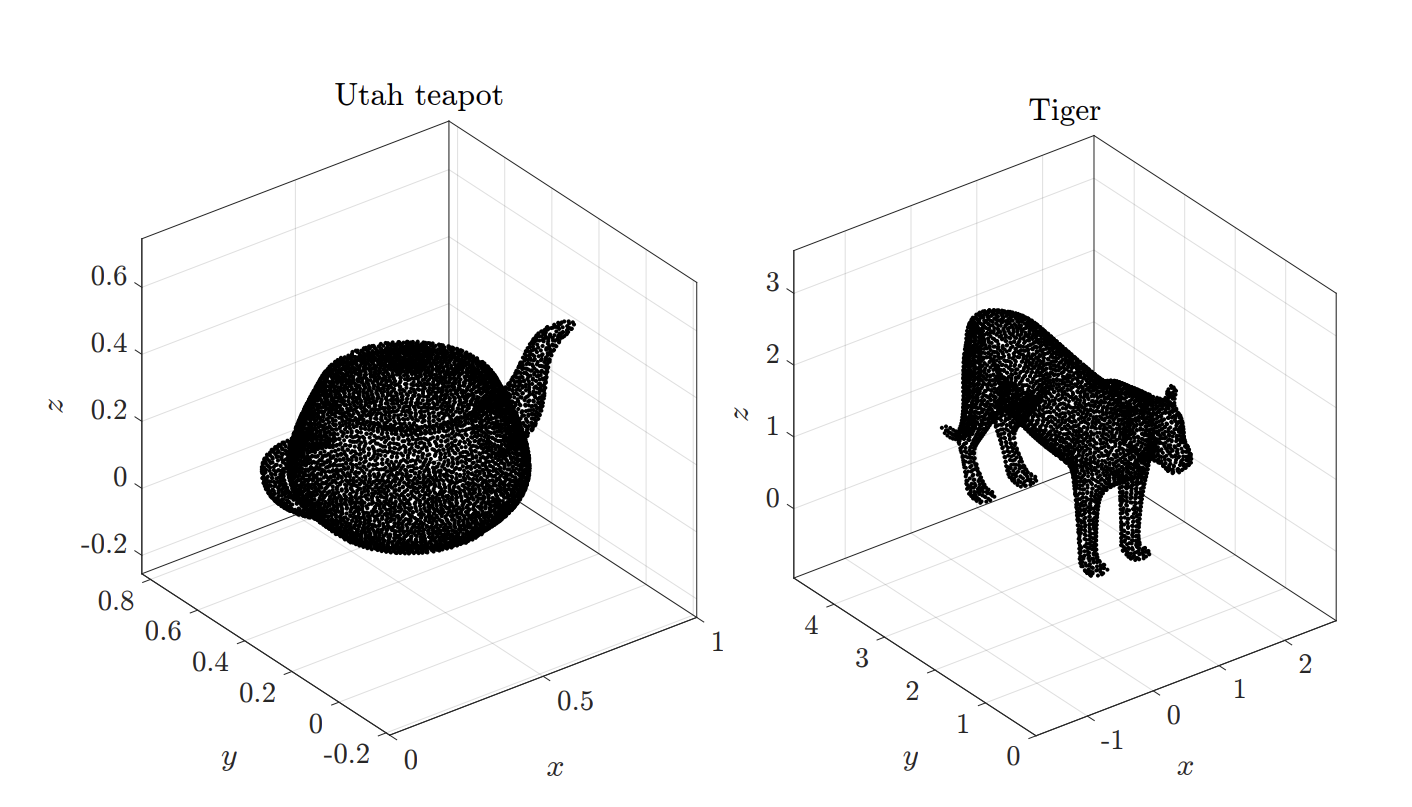
\includegraphics[width=\linewidth]{Slike/primeri.png}
\end{frame}
\begin{frame}
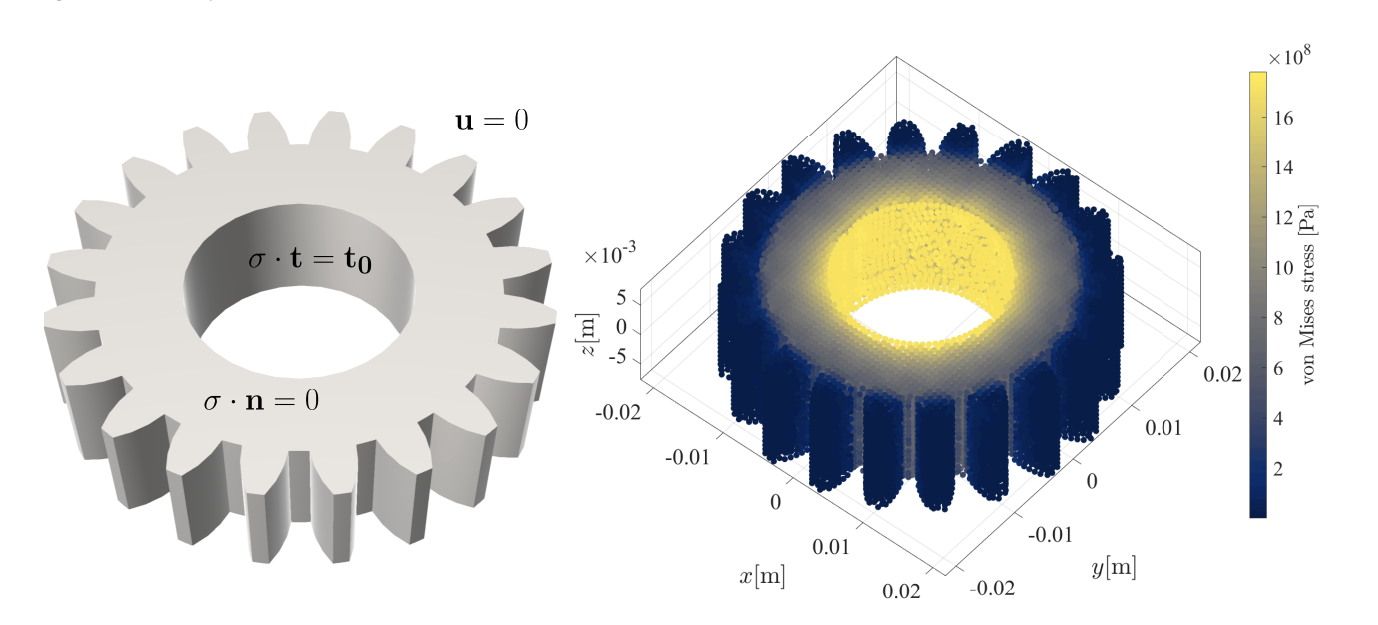
\includegraphics[width=\linewidth]{Slike/cog.png}
\end{frame}
\begin{frame}
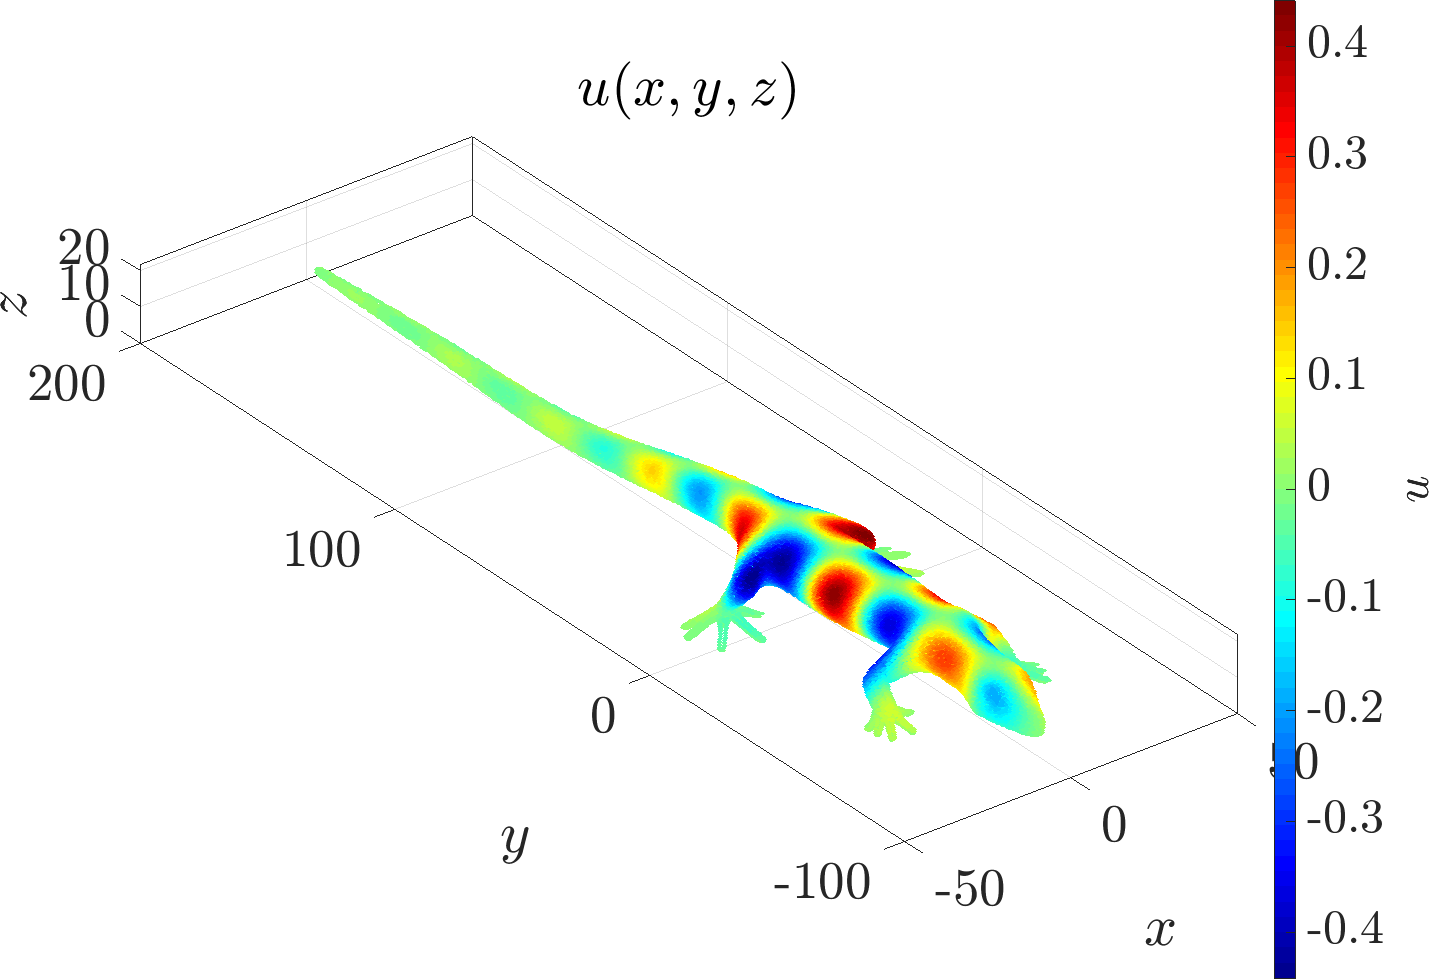
\includegraphics[width=\linewidth]{Slike/geko.png}
\end{frame}
\begin{frame}
\frametitle{Comparison}
\includegraphics[width=.6\linewidth]{Slike/nurbsDuck.png}
\includegraphics[width=.4\linewidth]{Slike/inRSDuck.png}
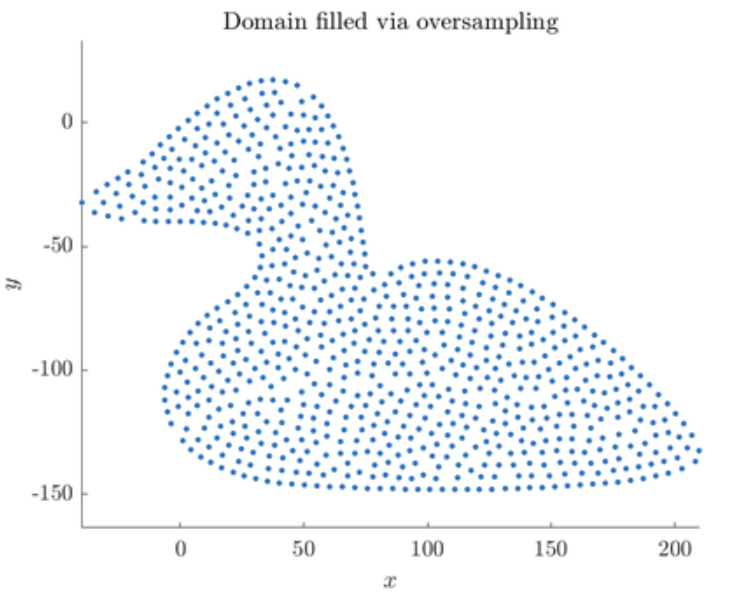
\includegraphics[width=.4\linewidth]{Slike/supersampling2.png}
\end{frame}
\end{document}